\pdfminorversion=4
\documentclass[aspectratio=169]{beamer}

\mode<presentation>
{
  \usetheme{default}
  \usecolortheme{default}
  \usefonttheme{default}
  \setbeamertemplate{navigation symbols}{}
  \setbeamertemplate{caption}[numbered]
  \setbeamertemplate{footline}[frame number]  % or "page number"
  \setbeamercolor{frametitle}{fg=white}
  \setbeamercolor{footline}{fg=black}
} 

\usepackage[english]{babel}
\usepackage{inputenc}
\usepackage{tikz}
\usepackage{courier}
\usepackage{array}
\usepackage{bold-extra}
\usepackage{minted}
\usepackage[thicklines]{cancel}
\usepackage{fancyvrb}

\xdefinecolor{ucred}{rgb}{0.50,0,0}
\xdefinecolor{dianablue}{rgb}{0.18,0.24,0.31}
\xdefinecolor{darkblue}{rgb}{0.1,0.1,0.7}
\xdefinecolor{darkgreen}{rgb}{0,0.5,0}
\xdefinecolor{darkgrey}{rgb}{0.35,0.35,0.35}
\xdefinecolor{darkorange}{rgb}{0.8,0.5,0}
\xdefinecolor{darkred}{rgb}{0.7,0,0}
\definecolor{darkgreen}{rgb}{0,0.6,0}
\definecolor{mauve}{rgb}{0.58,0,0.82}

\title[2025-09-11-jupyter-for-teaching]{\textcolor{black}{Jupyter for Teaching}}
\author{Jim Pivarski}
\institute{University of Chicago -- Data Science Institute}
\date{September 11, 2025}

\usetikzlibrary{shapes.callouts}

\begin{document}

\logo{\pgfputat{\pgfxy(0.11, 7.4)}{\pgfbox[right,base]{\tikz{\filldraw[fill=ucred, draw=none] (0 cm, 0 cm) rectangle (50 cm, 1 cm);}\mbox{\hspace{-8 cm}
\includegraphics[height=1 cm]{uchicago-logo-long.png}\hspace{0.1 cm}{
\includegraphics[height=1 cm]{dsi-logo-long.png}}\hspace{0.1 cm}}}}}

\begin{frame}
  \titlepage
\end{frame}

\logo{\pgfputat{\pgfxy(0.11, 7.4)}{\pgfbox[right,base]{\tikz{\filldraw[fill=ucred, draw=none] (0 cm, 0 cm) rectangle (50 cm, 1 cm);}\mbox{\hspace{-8 cm}
\includegraphics[height=1 cm]{uchicago-logo.png}{
\includegraphics[height=1 cm]{dsi-logo.png}}\hspace{0.1 cm}}}}}

% Uncomment these lines for an automatically generated outline.
%\begin{frame}{Outline}
%  \tableofcontents
%\end{frame}

% START START START START START START START START START START START START START

\begin{frame}{Big picture}
\Large
\vspace{0.5 cm}

I almost called this talk ``Literate Programming for Teaching,'' \\ because that's the paradigm.

\vspace{1 cm}
\uncover<2->{Jupyter is just the technology.}
\end{frame}

\begin{frame}{Behold, the ``Tioga'' code-editing environment from 1982!}
\vspace{0.2 cm}
\begin{columns}
\column{0.95\linewidth}
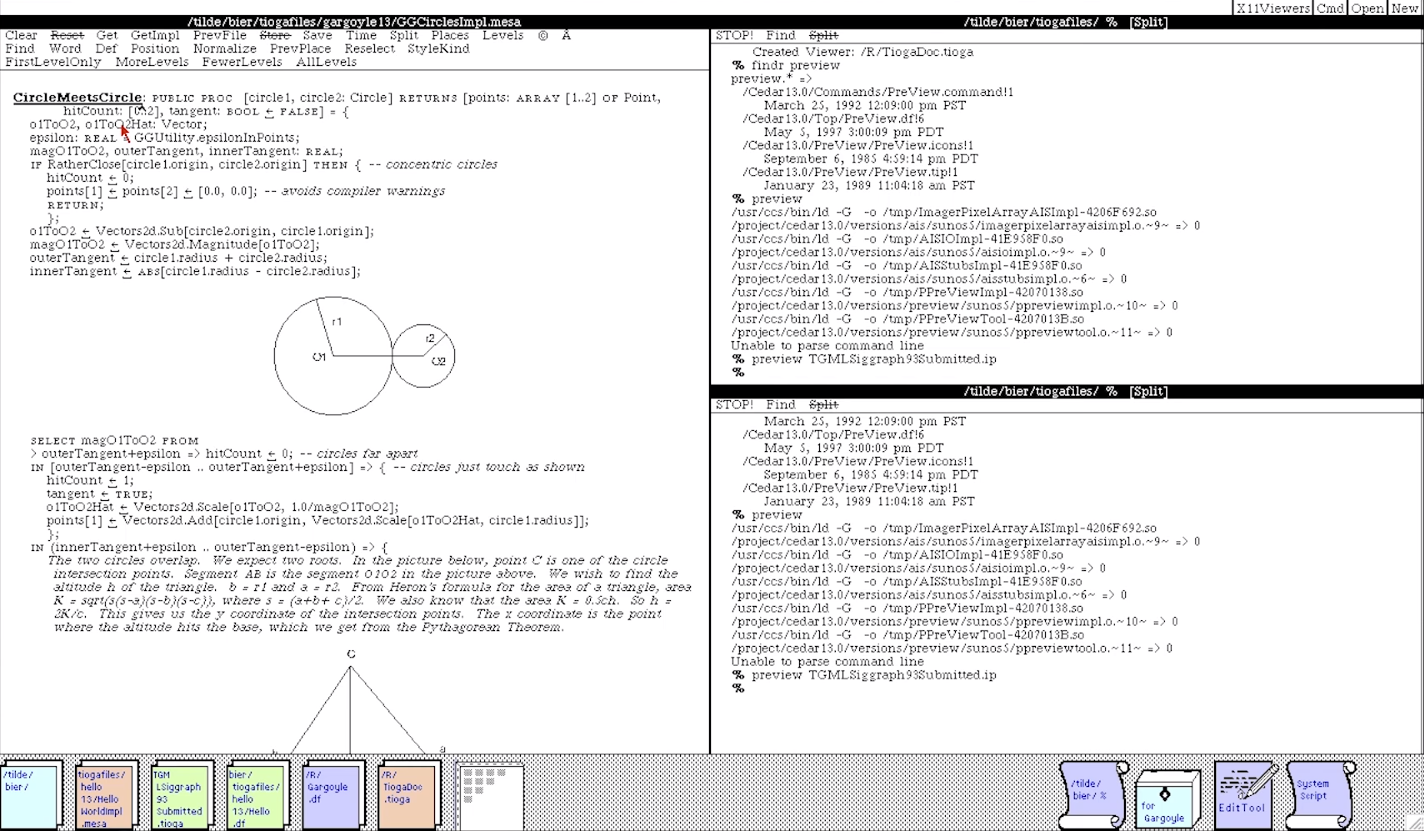
\includegraphics[width=\linewidth]{img/screenshot-1982-cedar-tioga.png}
\end{columns}
\end{frame}

\begin{frame}{Or ``MathCad'' for personal computers in 1986}
\vspace{0.2 cm}
\begin{columns}
\column{0.73\linewidth}
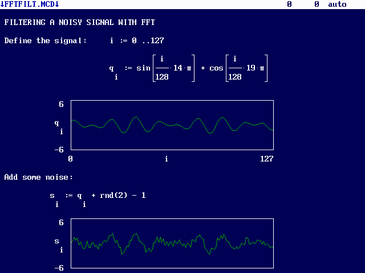
\includegraphics[width=\linewidth]{img/screenshot-1986-mathcad.png}
\end{columns}
\end{frame}

\begin{frame}{``Mathematica'' in 1987 was the first of these to be mainstream}
\vspace{0.2 cm}
\begin{columns}
\column{0.83\linewidth}
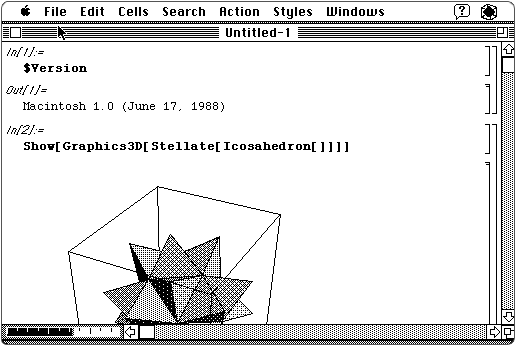
\includegraphics[width=\linewidth]{img/screenshot-1987-mathematica.png}
\end{columns}
\end{frame}

\begin{frame}{Jupyter wasn't even the first to use web browsers and Python}
\vspace{0.2 cm}
\begin{columns}
\column{0.54\linewidth}
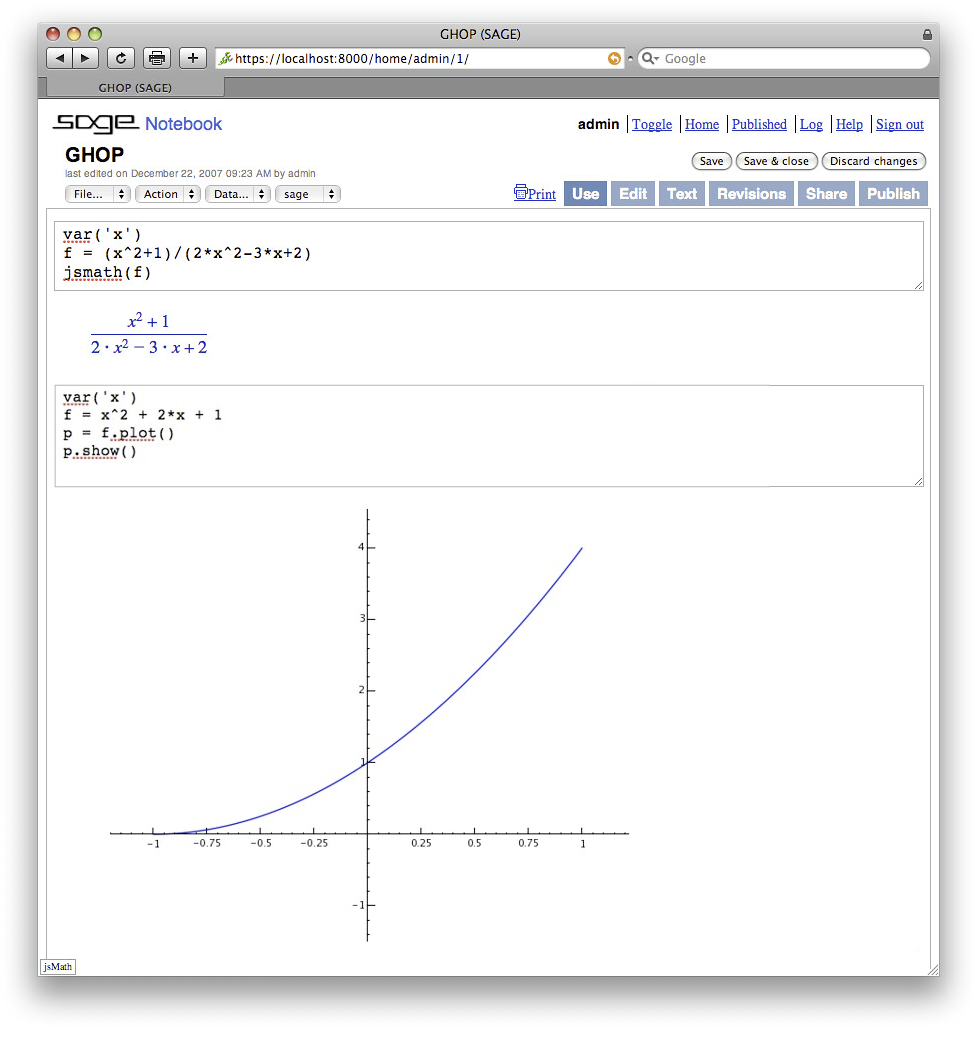
\includegraphics[width=\linewidth]{img/screenshot-2007-sage.png}

\column{0.38\linewidth}
\Large
This is ``SAGE'' in 2007.
\end{columns}
\end{frame}

\begin{frame}{Jupyter started life as ``IP[y]: Notebook'' in 2012}
\vspace{0.2 cm}
\begin{columns}
\column{0.6\linewidth}
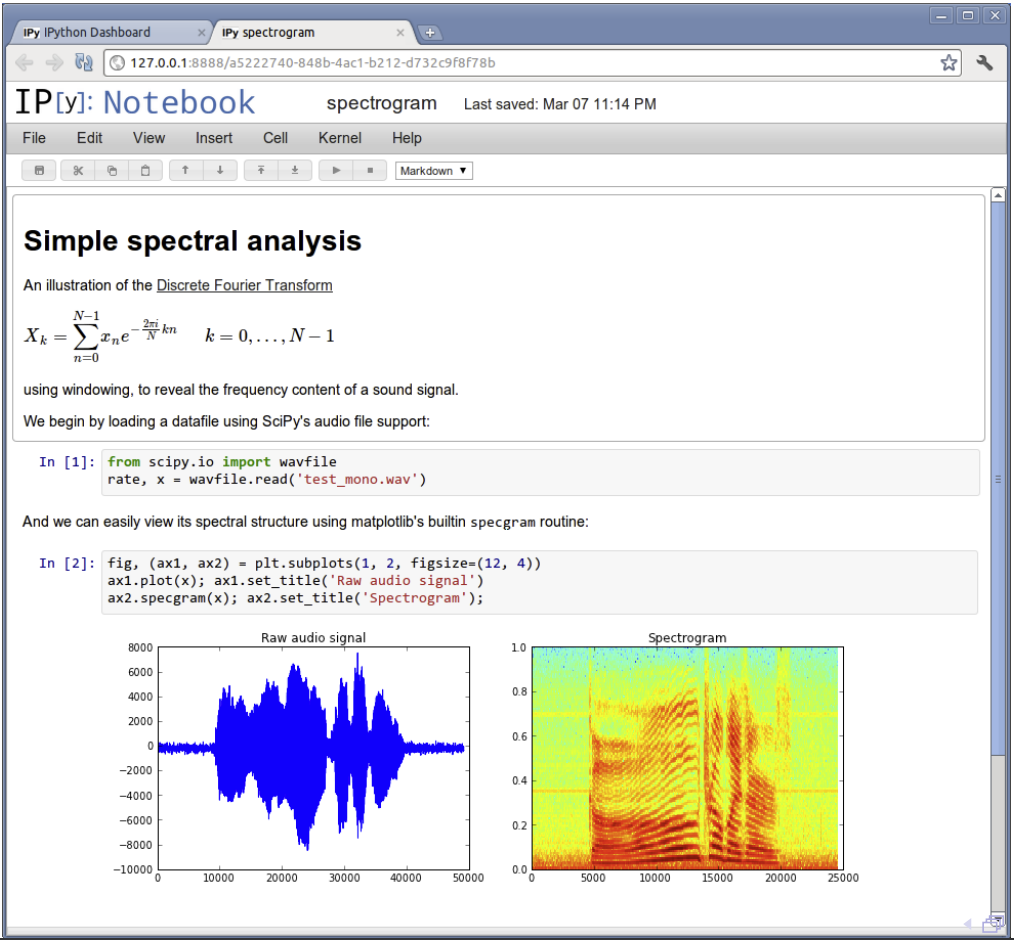
\includegraphics[width=\linewidth]{img/screenshot-2012-ipython-notebook.png}
\end{columns}
\end{frame}

\begin{frame}{But changed its name in 2015 to say it's for \textcolor{yellow}{\bf Ju}lia, \textcolor{yellow}{\bf Pyt}hon, and \textcolor{yellow}{\bf R}}
\vspace{0.2 cm}
\begin{columns}
\column{0.52\linewidth}
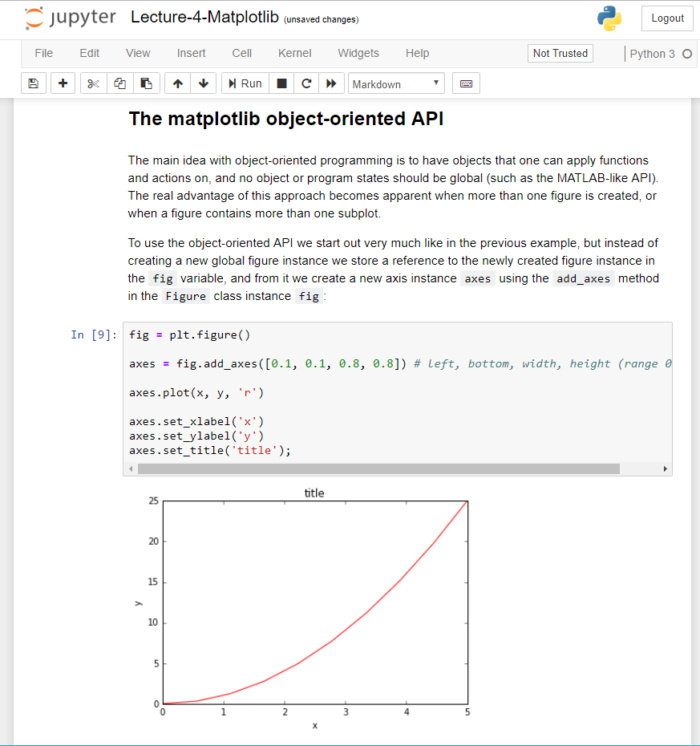
\includegraphics[width=\linewidth]{img/screenshot-2015-jupyter-notebook.png}

\column{0.5\linewidth}
\Large
\textcolor{gray}{(But now Julia programmers more often use Pluto.jl and R programmers often use RStudio.)}
\end{columns}
\end{frame}

\begin{frame}{Rewritten as a complete, Tioga-like environment in 2018: JupyterLab}
\vspace{0.2 cm}
\begin{columns}
\column{0.98\linewidth}
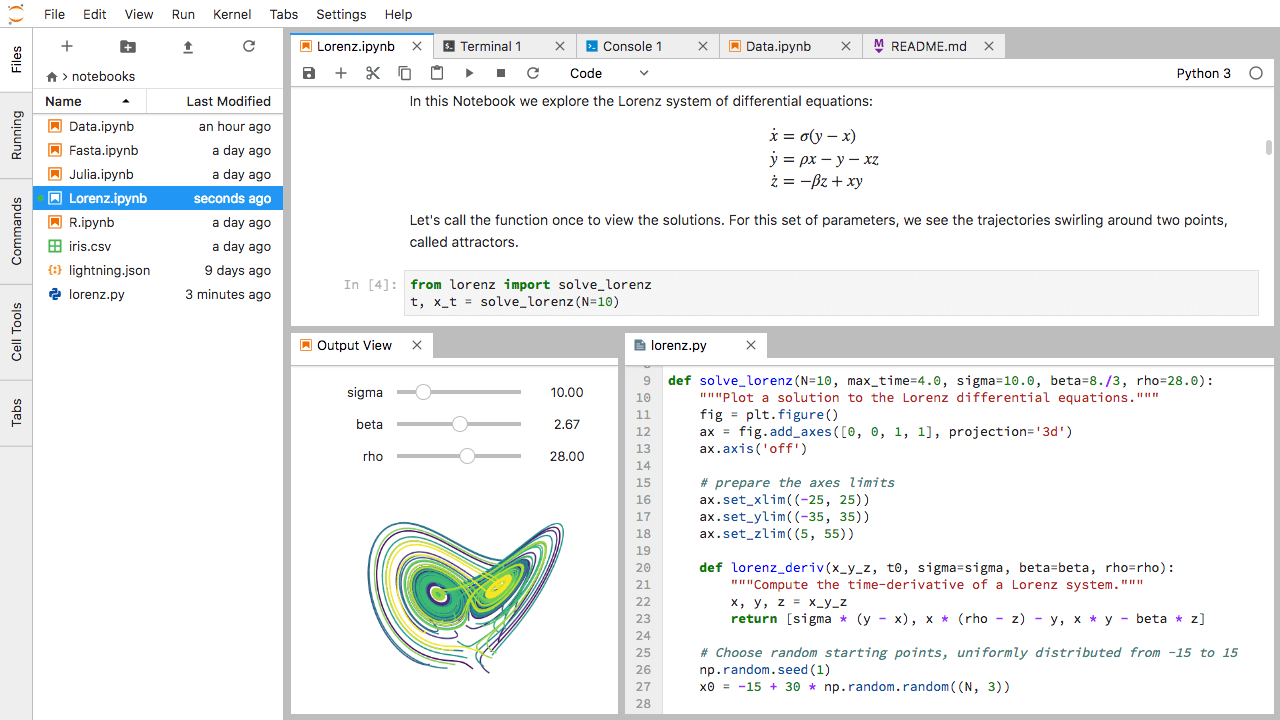
\includegraphics[width=\linewidth]{img/screenshot-2018-jupyterlab.png}
\end{columns}
\end{frame}

\begin{frame}{Notebooks are the middle of three fundamental types of code editors}
\vspace{0.2 cm}
\begin{columns}
\column{\linewidth}
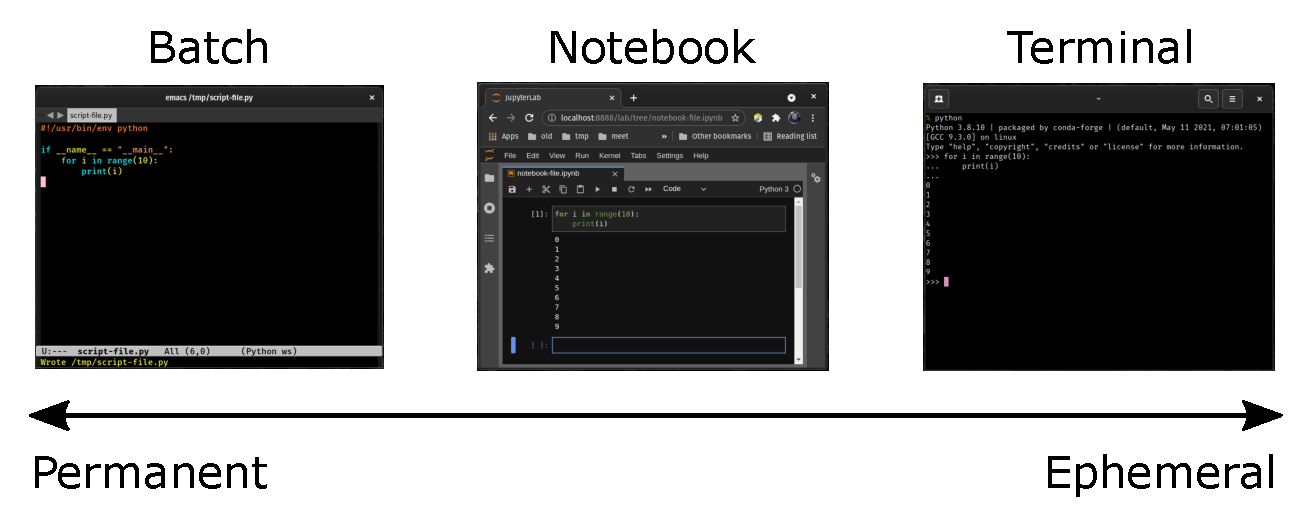
\includegraphics[width=\linewidth]{img/fundamental-3-modes-of-programming.pdf}
\end{columns}
\end{frame}

\begin{frame}{Batch: the most permanent}
\vspace{0.2 cm}
\begin{columns}
\column{0.45\linewidth}
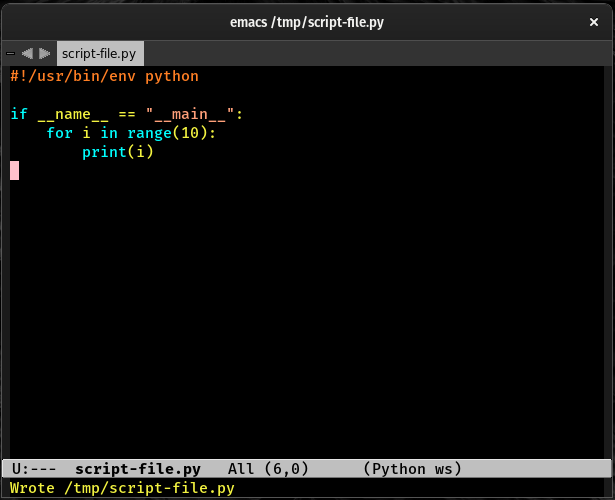
\includegraphics[width=\linewidth]{img/fundamental-3-modes-batch.png}

\column{0.5\linewidth}
\large
\begin{itemize}\setlength{\itemsep}{0.25 cm}
\item<1-> This is the oldest, from the punch-card, time-sharing era.
\item<2-> Best for developing software libraries, with an emphasis on architecture and the large scale.
\item<3-> Testing means running the whole program from its beginning (maybe even compiling it if you're using one of {\it those} languages).
\item<4-> Conceit: you're a sculptor, carving a beautiful ediface that will stand the test of time.
\end{itemize}
\end{columns}
\end{frame}

\begin{frame}{Terminal: the most ephemeral}
\vspace{0.2 cm}
\begin{columns}
\column{0.45\linewidth}
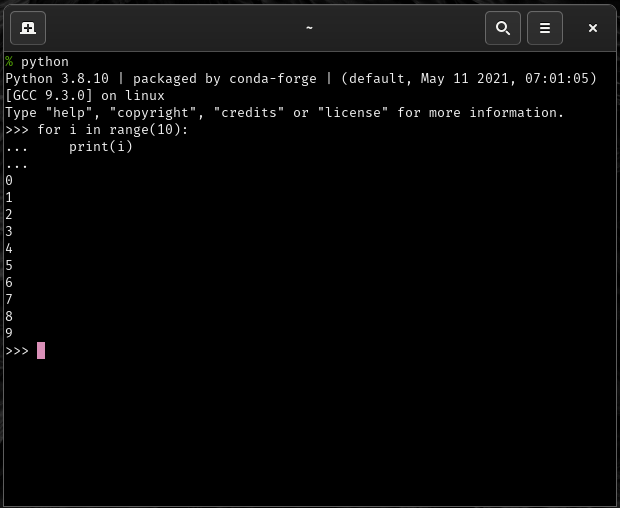
\includegraphics[width=\linewidth]{img/fundamental-3-modes-terminal.png}

\column{0.53\linewidth}
\large
\begin{itemize}\setlength{\itemsep}{0.25 cm}
\item<1-> Also has a long history in interactive languages like LISP, SPEAKEASY, and BASIC, as well as filesystem shells like UNIX and VAX.
\item<2-> Best for getting quick answers like, ``What are the first few elements of this list?'' or making simple changes like, ``Convert all the images in this directory to JPEG.''
\item<3-> Testing is continuous and immediate.
\item<4-> Conceit: you're a hack3r, mashing out commands at a breakneck pace.
\end{itemize}
\end{columns}
\end{frame}

\begin{frame}{Notebooks: in between}
\vspace{0.2 cm}
\begin{columns}
\column{0.45\linewidth}
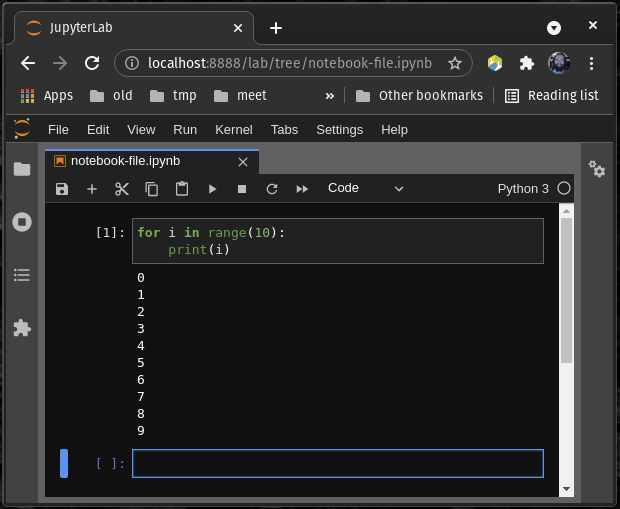
\includegraphics[width=\linewidth]{img/fundamental-3-modes-notebook.png}

\column{0.53\linewidth}
\large
\begin{itemize}\setlength{\itemsep}{0.25 cm}
\item<1-> Perceived as new, but they've had an important place in mathematical and data analysis software for almost as long as the spreadsheet.
\item<2-> Best for quick analyses that will likely be repeated: iterative investigation. Or for presenting code with detailed explanations, like a book, or teaching and running code in real-time.
\item<3-> Testing is continuous and immediate.
\item<4-> Conceit: Literate Programming!
\end{itemize}
\end{columns}
\end{frame}

\begin{frame}{Literate Programming}
\vspace{0.5 cm}
\begin{columns}
\column{1.03\linewidth}
I believe that the time is ripe for significantly better documentation of programs, and that we can best achieve this by considering programs to be works of literature. Hence, my title: ``Literate Programming.''

\hfill --- Donald Knuth, 1984

\vspace{1.2 cm}

\uncover<2->{One deliberately writes a paper, not just comments, along with code.}

\uncover<2->{\hfill --- Doug McIlroy, 1986}

\vspace{1.2 cm}

%% \uncover<3->{A traditional computer program consists of a text file containing program code. Scattered amongst the program code are comments which describe the various parts of the code. In literate programming, the emphasis is reversed. Instead of writing code containing documentation, the literate programmer writes documentation containing code.}
\uncover<3->{Instead of writing code containing documentation, the literate programmer writes documentation containing code.}

\uncover<3->{\hfill --- Ross Williams, 1987}
\end{columns}
\end{frame}

\begin{frame}{Example: the LIGO black hole discovery}
\vspace{1 cm}
\LARGE

\centering \textcolor{blue}{\url{https://github.com/minrk/ligo-binder/blob/master/index.ipynb}}

\end{frame}

\begin{frame}{Questions about the LIGO example}
\Large
\vspace{0.5 cm}
\begin{columns}
\column{1.03\linewidth}
Is it a good book?

\vspace{0.25 cm}
\uncover<2->{\textcolor{orange}{\bf Maybe, for an advanced student who's willing to put in effort.}}

\vspace{1 cm}
Is it a good lecture presentation? \uncover<3->{\textcolor{orange}{\bf \LARGE No!}}

\vspace{0.25 cm}
\begin{enumerate}
\item<4-> Font is too small; enlarging it would push too much off the screen.
\item<5-> As a vertical document, it's prone to scrolling too fast.
\item<6-> Too much code in the cells, hard to unpack.
\item<7-> Students can't start until they install the software and data files.
\end{enumerate}
\end{columns}
\end{frame}

\begin{frame}{``How to give a good Jupyter talk talk'' on YouTube}
\vspace{0.5 cm}
\begin{columns}
\column{1.1\linewidth}
\href{https://youtu.be/UhidS7fZZko?si=Vyr35fZhaSuyyxSW}{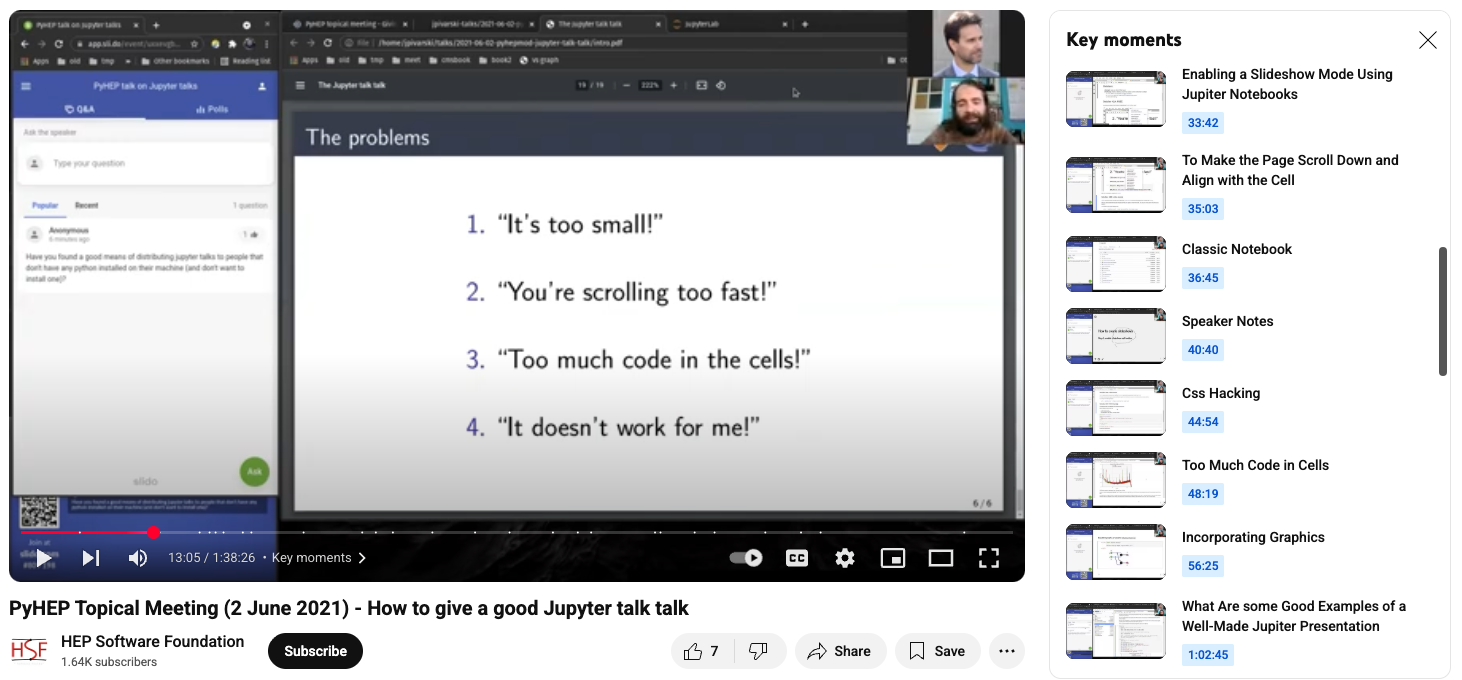
\includegraphics[width=\linewidth]{img/jupyter-talk-talk.png}}
\end{columns}
\end{frame}

\begin{frame}{All of the solutions I'll be presenting address these four problems}
\Large
\vspace{0.5 cm}
\begin{columns}
\column{0.58\linewidth}
\begin{enumerate}\setlength{\itemsep}{0.35 cm}
\item ``It's too small!''
\begin{itemize}
\item<2-> browser magnification
\item<2-> CSS hacks
\end{itemize}

\item ``You're scrolling too fast!''
\begin{itemize}
\item<2-> slide presentations: jupyterlab-deck
\item<2-> hiding hints and solutions
\end{itemize}

\item ``Too much code in the cells!''
\begin{itemize}
\item<2-> self-restraint?
\item<2-> mini-libraries
\end{itemize}

\item ``It doesn't work for me!''
\begin{itemize}
\item<2-> Docker
\item<2-> Binder
\item<2-> Codespaces
\item<2-> JupyterLite
\end{itemize}
\end{enumerate}
\end{columns}
\end{frame}

\begin{frame}{Before we get into it: how much interactivity are you going for?}
\Large
\vspace{0.5 cm}
\begin{columns}
\column{0.09\linewidth}
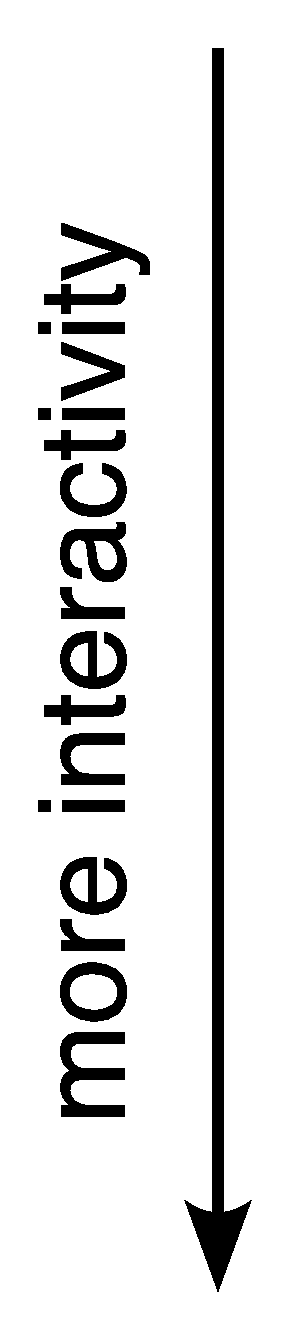
\includegraphics[width=\linewidth]{img/more-interactivity.pdf}

\column{0.9\linewidth}
The students watch pre-evaluated slides.

\vspace{0.5 cm}
The students watch you evaluate the cells.

\vspace{0.5 cm}
The students press ``shift-enter'' along with you.

\vspace{0.5 cm}
You stop now and then to ask, ``what if I do {\it this} instead?''

\vspace{0.5 cm}
You include formal exercises in the talk (short or long).
\end{columns}
\end{frame}

\begin{frame}{}
\LARGE
\vspace{1 cm}

\centering Next stop: the Dockerfile

\end{frame}

\end{document}
